%!TEX root = sandReportSpec.tex

\appendix


\chapter{Examples}
\label{chap:examples}


\section{Basic functionalities for spec 0.2}
\todo{Do we want to call this out as 0.2 even though we're not releasing 0.2?}

\subsection{DARMA environment}
Example showing how to initialize and finalize the DARMA environment.
\lstinputlisting[style=CppCodeNumbstyle]{../../examples/0.2/spec02individualFunctionalities/initAndFinalize.cc}

\subsection{DARMA rank and size}
Example showing DARMA rank and size.
\lstinputlisting[style=CppCodeNumbstyle]{../../examples/0.2/spec02individualFunctionalities/rankAndSize.cc}

\subsection{Deferred work creation}
Example showing a very simple \texttt{create\_work} with no dependencies.
\lstinputlisting[style=CppCodeNumbstyle]{../../examples/0.2/spec02individualFunctionalities/cw1.cc}

\subsection{Creating handles 1}
Example showing the use of \texttt{initial\_access}.
\lstinputlisting[style=CppCodeNumbstyle]{../../examples/0.2/spec02individualFunctionalities/initialAccess.cc}

\subsection{Creating handles 2}
Another example on \texttt{initial\_access} handle and its use.
\lstinputlisting[style=CppCodeNumbstyle]{../../examples/0.2/spec02individualFunctionalities/accessHandle1.cc}

\subsection{Arrow operator for handles}
Example showing the arrow operator on an handle.
\lstinputlisting[style=CppCodeNumbstyle]{../../examples/0.2/spec02individualFunctionalities/accessHandleArrowOperator.cc}

\subsection{Deferred work and constraining privileges}
Example showing how to issue a \texttt{create\_work} and constraining privileges on a handle to be read-only.
\lstinputlisting[style=CppCodeNumbstyle]{../../examples/0.2/spec02individualFunctionalities/cwReadsArg.cc}





\section{Hello World}

Example for one possible implementation of ``hello world''. 
There are three main parts involved: 
\begin{enumerate}
\item the DARMA environment is initialized, 
\item each rank issues a task to store a greeting message into a string, and
\item each rank then creates a task to printing to standard output the message and its rank.
\end{enumerate}
\lstinputlisting[style=CppCodeNumbstyle]{../../examples/0.2/darma_hello/darma_hello.cc}




\section{Key-Value Example}

This example is to illustrate simple transactions with the key-value store, 
but in a distributed setting. We will ask each rank to publish a float to be
read by two readers, a rank on the left and one on the right. Then we will ask
each rank to get two floats, those published by the left and right neighbors
and print to screen. We use periodic logic for neighbors.

\lstinputlisting[style=CppCodeNumbstyle]{../../examples/0.2/simple_kv/publish_get_parallel.cc}





\subsection{Publishing and read access}

This example explains in more detail the use of \texttt{publish} 
and \texttt{read\_access}. The example involves two DARMA ranks, each creating 
data, publishing it, and then fetching the other rank's data.

\lstinputlisting[style=CppCodeNumbstyle]{../../examples/0.2/spec02individualFunctionalities/publishAndReadAccess.cc}






\section{Publishing, versioning and lifetime of handles}

Lifetime of handles is tricky, particularly for \texttt{read\_access} type handles.  
In the following example, we initialize data, publish it, fetch it from another rank, 
modify the data, publish it again under a new version, and then fetch the new version from another rank. 
The \texttt{create\_work} on lines $64-68$ can't execute until the back end knows the first fetched version is no longer in use.
We put an extra set of \texttt{\{ \}} around the code in lines $40-61$ to tell the back end that 
the \texttt{readHandle} is no longer needed and can go out-of-scope and the fetching is done.

Without the scoping \texttt{\{\}}, the code would deadlock.
\texttt{darma\_finalize()} cannot return until after {\it all} the \texttt{create\_works} have completed.
However, without the additional scoping, the backend would not know that the first fetched version is no longer needed until \texttt{darma\_main()} returns, which requires \texttt{darma\_finalize()} to have already returned.

While scoping is necessary in this case, there will be other cases where it only helps to improve efficiency and concurrency 
in the scheduling and execution of tasks. Scoping is a good programming practice.


\lstinputlisting[style=CppCodeNumbstyle]{../../examples/0.2/spec02individualFunctionalities/version.cc}







\section{1D Poisson Equation}

Boundary value problem:

\begin{equation} 
  \frac{\partial^2 u(x)}{\partial x^2} = f(x) \quad 
  \text{in} \ \Omega=(0,1), \ \text{with} 
  \ u(0)=0, \ u(1)=\exp{(1)}\sin{(1)}
\end{equation} 
where $f(x)=2\exp{(x)}\sin{(x)}$. This problem is chosen because 
it has an exact solution, namely $u_{exact} = \exp{(1)}\sin{(1)}$. 
The exact solution will be used for checking the correctness 
of the code.

Discretize the domain with $N$ equally spaced points such that 
\begin{equation}
u_i \approx u(x_i), \quad f_i=f(x_i) 
\quad x_i = i \Delta x, \ \Delta x=\frac{1}{N-1}, \ \ i=0,1,...,N-1
\end{equation}
Use central difference approximation for the second derivative 
for all interior points:
\begin{large}
\begin{equation}
\begin{cases}
  \frac{u_{i+1} - 2u_i + u_{i-1}}{(\Delta x)^2}=f_i, & \text{for } i=1,...,N-2 \\
    u_0=0, \ u_{N-1}=\exp{(1)}*\sin{(1)} & \text{Dirichlet BC}
\end{cases}  
\end{equation}
\end{large}

This translates to a linear system of equations $Au=f$ 
where $A$ is an $N-2 \times N-2$ tridiagonal matrix 
\begin{equation}
A = \begin{vmatrix}
-2 & 1 \\
1 & -2 & 1 \\
& 1 & -2 & 1 \\
& & \ddots & \ddots & 1 \\
& & & 1 & -2
\end{vmatrix}.
\end{equation}

and $u$ is the unknown, and $f$ is the right-hand-side. 
Both $u$ and $f$ have size $N-2$. 
Solving this linear system yields the solution at all the inner 
points of the domain. For demonstration purposes, we solve 
this system using Thomas algorithm, a method well-suited 
for tridiagonal systems. 
The solver needs these vectors:
\begin{enumerate}
\item $a$: contains all the sub-diagonal entries. 
\item $b$: contains all the diagonal entries. 
\item $c$: contains all the upper-diagonal entries. 
\item $d$: contains all the right-hand-side entries. 
Also, our current version of the solver is 
such that on exit, the vector $d$ contains the solution.
\end{enumerate}

How do we implement this in DARMA? 
For demonstration purposes, we limit our attention to the case 
of a single rank. More complex examples involving multiple ranks will be shown later. 

There are three main steps involved, namely initialization, 
solution of the linear system, and error checking. 
The DARMA main file is as follows:
\lstinputlisting[style=CppCodeNumbstyle]{../../examples/0.2/poisson_1d_thomasAlgorithm/single_rank/single_rank.cc}

The header file constants.h contains:
\lstinputlisting[style=CppCodeNumbstyle]{../../examples/0.2/poisson_1d_thomasAlgorithm/constants.h}

The initialization function has the form:
\lstinputlisting[style=CppCodeNumbstyle]{../../examples/0.2/poisson_1d_thomasAlgorithm/single_rank/initialize.h}

The function to solve the linear system is:
\lstinputlisting[style=CppCodeNumbstyle]{../../examples/0.2/poisson_1d_thomasAlgorithm/single_rank/solveTridiag.h}

Finally, we check for convergence by checking the $L^1$-norm of the 
error between the computed and true solution.
\lstinputlisting[style=CppCodeNumbstyle]{../../examples/0.2/poisson_1d_thomasAlgorithm/single_rank/checkError.h}





\section{1D Heat Equation}

In this section, we solve the following simple problem:

\begin{equation} 
	\frac{\partial T(x,t)}{\partial t} = 
  \alpha \frac{\partial^2 T(x,t)}{\partial x^2} \quad 
  \text{in} \ \Omega=(0,1), \ \text{with} 
  \ T(0,t)=100, \ T(1,t)=10, \ \forall t \geq 0
\end{equation} 
where $T(x,t)$ is the temperature, $t$ is time, and $\alpha$ is the 
thermal diffusivity. The steady-state solution of this problem is 
a straight line connecting the left and right boundary conditions. 

We discretize the spatial domain with $N$ equally spaced points such that 
\begin{equation}
x_i = i \Delta x, \quad \Delta x=\frac{1}{N-1}, \quad \ i=0,1,...,N-1
\end{equation}
Similarly, in time with $n_{iter}$ steps such that 
\begin{equation}
t_m = m \Delta t, \quad \Delta t=\frac{t_{max}}{n_{iter}-1}, \quad \ m=0,1,...,n_{iter}-1
\end{equation}


We use second-order finite-differences in space, and Euler method in time. 
Hence, the discrete version takes the form: 
\begin{large}
\begin{equation}
\frac{T_i^{m+1} - T_i^m}{\Delta t} 
= \alpha \frac{T_{i+1}^m - 2T_i^m + T_{i-1}^m}{\Delta x^2}
\end{equation}
\end{large}
where $T_i^m$ represents the approximate temperature at the $i$-th grid point, 
at the $m$-th time instant. Hence, for every grid point $i$, given the solution 
at the current time instant $T_i^m$, the solution at the next step is given by 
\begin{large}
\begin{equation}
T_i^{m+1} = T_i^m + \frac{ \alpha \Delta t }{\Delta x^2} 
(T_{i+1}^m - 2T_i^m + T_{i-1}^m)
\end{equation}
\end{large}

For demonstration purposes, we adopt here $\alpha=0.0075$, discretize the domain 
with $N=16$, use $n_{iter}=2500$ time steps and consider $\Delta t=0.05$ which is 
sufficiently small for the numerical method to be stable.
The main constants are defined in the following header file:
\lstinputlisting[style=CppCodeNumbstyle]{../../examples/0.2/heat_1d/common_heat1d.h}

The problem involves three main stages, namely initialization, time advancing, 
and convergence check. We use four DARMA ranks to distribute the grid points, 
such that each rank handles a local grid with $4$ points. 
In brief, the problem is setup by having each rank 
generate tasks for its local grid, then communicate with the neighboring ranks 
to get the information for the ghost points needed to update the stencil. 
A high-level schematic of the work-flow is shown in Figure~\ref{fig:example_heat1d}.

\begin{figure}[!ht]
\centering
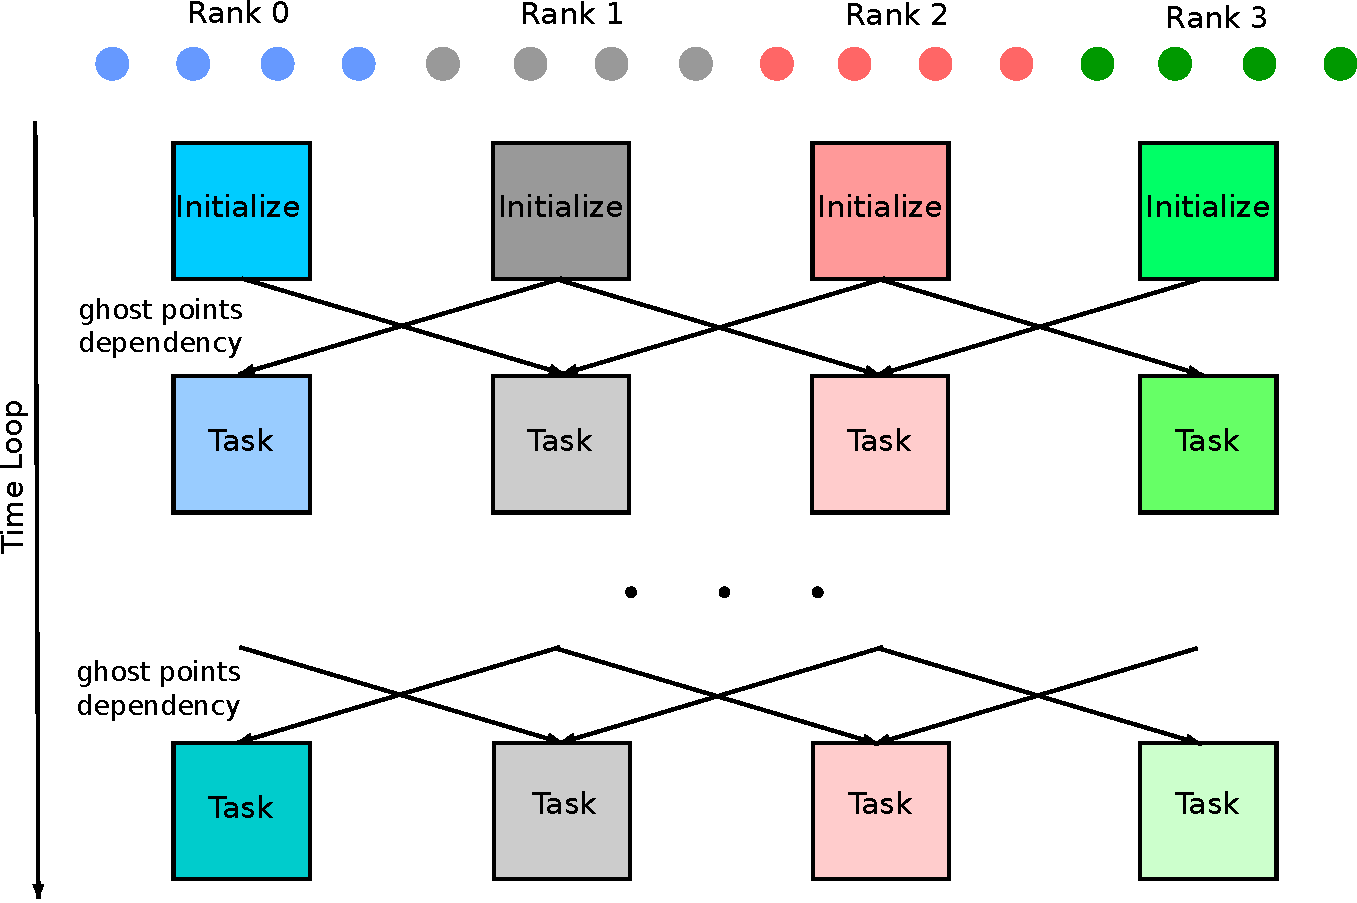
\includegraphics[width=0.75\textwidth]{./figures/examples/heat_tasks.pdf}
\caption{Schematic of task generation for the heat 1D PDE.}
\label{fig:example_heat1d}
\end{figure}


The full main code is shown below.
\lstinputlisting[style=CppCodeNumbstyle]{../../examples/0.2/heat_1d/heat_1D_darma_simple/heat_1d_darma_simple.cc}





